\chapter{CONSIDERAÇÕES FINAIS}
\thispagestyle{empty}

Ao consultar o Portal de Inovação e Diretório de dados do CNPq, é possível notar que o Brasil possui inúmeros pesquisadores em diversas áreas do conhecimento, bem como diversos projetos de pesquisa, incubadoras e parques tecnológicos dignos de primeiro mundo.

Este trabalho apresentadou uma leve perspectiva sobre um novo plano de ação do governo brasileiro envolvendo as novas IF, reformuladas e focadas em ensino de qualidade, e de Polos de Inovação, idealizados para reger as relações estabelecidas entre os institutos e as empresas locais onde estão localizados.

Visto a importância notada pela relação UEG ao redor do país, este estudo ainda visa destacar a necessidade de um acompanhamento do desenvolvimento da relação IF-Polo de Inovação, para avaliar o impacto desta na sociedade e na transferência de tecnologia para empresas locais.

\section{CRONOGRAMA}

\begin{enumerate}
  \item{Contato – Equipe Administrativa do Polo de Inovação Campos dos Goytacazes (PICG);}
  \item{Participação na criação do Escritório de Projetos do PICG;}
  \item{Revisão Bibliográfica;}
  \item{Apresentação do Projeto;}
  \item{Roteirização;}
  \item{Coleta de dados – através do escritório de projetos – Empresas Associadas;}
  \item{Resultado e Discussões;}
  \item{Revisão do projeto final;}
  \item{Defesa.}
\end{enumerate}

\begin{figure}[ht]
  \centering
  \scalebox{0.7}{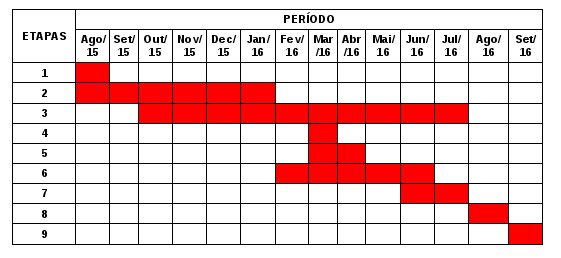
\includegraphics{figuras/cronograma}}
  \caption{Cronograma seguido pelo projeto}
  \label{crescimento_odf}
\end{figure}

\begin{table}
  \caption{Dummy table}
  \begin{tabular}{|l||l|l||l|l|}
    \hline
     &\multicolumn{2}{l|}{Singular}&\multicolumn{2}{l|}{Plural}\\
    \cline{2-5}
     &English&\textbf{Gaeilge}&English&\textbf{Gaeilge}\\
    \hline\hline
    1st Person&at me&\textbf{agam}&at us&\textbf{againn}\\
    2nd Person&at you&\textbf{agat}&at you&\textbf{agaibh}\\
    3rd Person&at him&\textbf{aige}&at them&\textbf{acu}\\
     &at her&\textbf{aici}& & \\
    \hline
  \end{tabular}
\end{table}
